\documentclass[9pt,twocolumn,twoside]{../../styles/osajnl}
\usepackage{fancyvrb}
\journal{i524}

\title{Naiad}

\author[1,*]{Rahul Raghatate}
\author[1]{Snehal Chemburkar}

\affil[1]{School of Informatics and Computing, Bloomington, IN 47408,
  U.S.A.}

\affil[*]{Corresponding authors: rragahta@iu.edu, snehchem@iu.edu }

\dates{paper-2, \today}

\ociscodes{Naiad, iterative, dataflow, graph, stream}

% replace this with your url in github/gitlab
\doi{\url{https://github.com/cloudmesh/sp17-i524/blob/master/paper2/S17-IR-2026/report.pdf}}


\begin{abstract}
Naiad is a distributed system based on computational model called
timely dataflow developed for execution of data-parallel, cyclic
dataflow programs. It provides an in-memory distributed dataflow
framework which exposes control over data partitioning and enables
features like the high throughput of batch processors, the low latency
of stream processors, and the ability to perform iterative and
incremental computations \cite{paper1-Naiad}. These features allow the
efficient implementation of many dataflow patterns, from bulk and
streaming computation to iterative graph processing and machine
learning.  This paper explaines the Naiad Framework, its abstractions,
and the reasoning behind it.
\newline
\end{abstract}

\setboolean{displaycopyright}{true}

\begin{document}

\maketitle

\TODO{This review document is provided for you to achieve your
  best. We have listed a number of obvious opportunities for
  improvement. When improving it, please keep this copy untouched and
  instead focus on improving report.tex. The review does not include
  all possible improvement suggestions and for each comment you may
  want to check if it applies elsewhere in the document.}

\TODO{Assessment: Some revisions suggested. Please address the review
  comments below.}

\TODO{Abstract: Very good. The citation in the abstract is unnecessary
  and should be put in the main text.}

\TODO{Your Introduction can be improved significantly. Currently, it
  is not very clear, it repeats some points, and it doesn't give a
  good overview of the problem domain.}

\TODO{The flow of the paper could be improved as well. Some of the
  sections stand on their own, without you motivating why they're
  there, or how they relate to other sections of the paper.}

\TODO{In general, please always include a space following punctuation
  such as periods, commads, colons, etc.}

\section{Introduction}

Abundance of distributed dataflow systems around the big data
ecosystem has resulted in achieving many goals like high throughput,
incremental updating, low latency stream processing, iterative
computation. Many graph analytics procedures involves incremental as
well as iterative processing. However, most data-parallel systems
support either incremental update or iteration, but not both.

\TODO{Please ellaborate what incremental vs iterative processing
  is. Include an example. This is critical to understanding the
  problem domain, so you need to make sure the reader is on board.}

Frameworks like descendants of MapReduce
\cite{paper-incoop,paper-nectar},stream processing systems
\cite{eventstream,paper-spade}, materialized view-maintenance engines
\cite{paper-maintainance}, provide efficient support for incremental
input, but do not support iterative processing. On the other hand,
iterative data-parallel frameworks like Datalog \cite{paper-datalog},
recursive SQL databases \cite{paper-SQL} and systems adding iteration
over MapReduce like model
\cite{paper-haloop,paper-twister,paper-ceil,paper-RDD} provide a
constrained programming model (e.g. stratified negation in Datalog)
and none supports incremental input processing \cite{paper2-Naiad}.

Map Reduce \TE, being functional language,requires passing the entire
state of the graph from one stage to the next, which is
inefficient. \TODO{This sentence is not clear, and is in some parts
  incorrect. MapReduce not a language. And why do you call it
  functional? What graph and stages are you discussing? This is very
  unclear and needs more context.} In real-time applications batch
processing delays of MapReduce may prove unacceptable
\cite{www-informationage-blog-wordpress-naiad}.

With a goal to find common low-level abstraction and system design
that could be re-used for all of these computational workloads and to
reduce the engineering cost of domain-specific distributed systems by
allowing them to share a single highly optimized core codebase, Naiad,
a timely dataflow system was developed at Microsoft by Derek G. Murray
\textit{et al.} \cite{paper3-Naiad}. \TODO{Try to write shorter sentences. It makes the paper easier to read and undestand.}

Naiad extends standard batch data-parallel processing models like
MapReduce, Hadoop, and Dryad/DryadLINQ, to support efficient
incremental updates to the inputs in the manner of a stream processing
system, while at the same time enabling arbitrarily nested fixed-point
iteration \cite{paper1-Naiad}.

Naiad, a distributed system for executing data parallel cyclic
dataflow programs offers high throughput batch processing, low latency
stream processing and the ability to perform iterative and incremental
computations all in one framework \cite{www--blog-huula-review-naiad}.

In Naiad, the underlying computation framework provides a mechanism
for iteration and incremental update, while the language provides a
structured means of expressing these computations. This yields both an
expressive programming model and an efficient implementation
\cite{paper2-Naiad}.

\TODO{The last three paragraphs are very disjointed without a clear
  link between them. The second to last paragraph actually repeats
  things you've already said.}

\TODO{Please improve clarity and organization of the whole Intro
  section. Start with an example problem and how a purely incremental
  or purley iterative system wouldn't solve it. Then talk about Naiad
  like you have, but organize your paragraphs better.}

\section{Architecture}

The Naiad architecture consists of two main components- (1)
incremental processing of incoming updates and (2) low-latency
real-time querying of the application state.
\begin{figure}[htbp]
\centering
\fbox{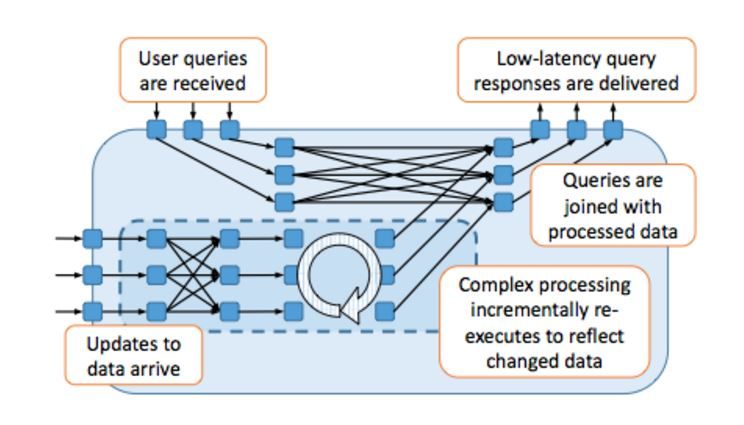
\includegraphics[width=\linewidth]{images/Naiad_application.JPG}}
\caption{Naiad Application that support real time querries on
  continually updated data \cite{paper1-Naiad}.}
\label{Naiad-arch}
\end{figure}

Many data processing tasks require low-latency interactive access to
results, iterative sub-computations, and consistent intermediate
outputs so that sub-computations can be nested and composed. \TODO{This sentence is out of scope for this section. It belongs in the Intro perhaps.} Figure
\ref{Naiad-arch} shows a Naiad application that supports realtime
queries on continually updated data. The dashed rectangle represents
iterative processing that incrementally updates as new data arrive
\cite{paper1-Naiad}.

From Figure \ref{Naiad-arch}, it can be seen that query path is
clearly separated from the update path. This results in query
processing separately on a slightly stale version of the current
application state and the query path does not get blocked or incur
delays due to the update processing. This also resolves complex
situations: If queries shared the same path with updates, the queries
could be accessing partially processed/incomplete/inconsistent states,
which would have to be taken care out separately.

Even though hybrid approach to assemble the application in Figure
\ref{Naiad-arch} by combining multiple existing systems have been
widely deployed, applications built on a single platform as in Figure
\ref{Naiad-arch} are typically more efficient, succinct, and
maintainable \cite{paper1-Naiad}.

\subsection{Features} 
Naiad being a timely dataflow computational model, enriches dataflow
computation with timestamps that represent logical points in the
computation and provide the basis for an efficient, lightweight
coordination mechanism.Timely dataflow supports the following three
features:

\begin{enumerate}
\item Structured loops allowing feedback in the dataflow
\item Stateful dataflow vertices capable of consuming and producing
  records without global coordination, and
\item Notifications for vertices once they have received all records
  for a given round of input or loop iteration.
\end{enumerate}

Structured loops and Stateful dataflow vertices allows iterative and
incremental computations with low latency.Notifications makes Naiad
possible to produce consistent results, at both outputs and
intermediate stages of computations, in the presence of streaming or
iteration \cite{paper1-Naiad}.

\section{Timely dataflow}

\TODO{Please, improve the flow of the paper. How does this section
  relate to any of the sections preceding it?}

Applications should produce consistent results, and consistency
requires coordination, both across dataflow nodes and around loops
\cite{paper1-Naiad}. Timely dataflow is a computational model that
attaches virtual timestamps to events in structured cyclic data-flow
graphs providing coordination mechanism that allows low-latency
asynchronous message processing while efficiently tracking global
progress and synchronizing only where necessary to enforce
consistency. Naiad model simply checkpoints its state periodically,
restoring the entire system state to the most recent checkpoint on
failure. Even if its \TODO{Know the difference between "its" and "it
  is"} not a sophisticated design,it was chosen in part for its low
overhead. Faster common-case processing allows more computation to
take place in the intervals between checkpointing, and thus often
decreases the total time to job completion \cite{paper3-Naiad}.

\subsection{Asynchronous messaging}
All dataflow models require some communication means for message
passing between node over outgoing edges. In a timely dataflow system,
each node implements an \textit{OnRecv} event handler that the system
can call when a message arrives on an incoming edge, and the system
provides a \textit{Sendmethod} that a node can invoke from any of its
event handlers to send a message on an outgoing edge
\cite{paper3-Naiad}. Messages are delivered asynchronously.

\subsection{Consistency}
Computations like reduction functions \textit{Count} or
\textit{Average} include subroutines that must accumulate all of their
input before generating an output. At the same time, distributed
applications commonly split input into small asynchronous messages to
reduce latency and buffering. For timely dataflow to support
incremental computations on unbounded streams of input as well as
iteration, it has a mechanism to signal when a node (or data-parallel
set of nodes) has seen a consistent subset of the input for which to
produce a result \cite{paper3-Naiad}.

\subsection{Iterative Graph Dataflow}
A Naiad dataflow graph is acyclic apart from structurally nested
cycles that correspond to loops in the program. The logical timestamp
associated with each event represents the batch of input that the
event is associated with, and each subsequent integer gives the
iteration count of any (nested) loops that contain the node. Every
path around a cycle includes a special node that increments the
innermost coordinate of the timestamp.  The system enforced rule
restricts event handler from sending a message with a time earlier
than the timestamp for the event it is handling ensuring a
\textit{partial order} on all of the pending events (undelivered
messages and notifications) in the system,thus enabling efficient
progress tracking \cite{paper1-Naiad}.


\subsection{Progress Tracking}
The ability to deliver notifications(an event that fires when all
messages at or before a particular logical timestamp have been
delivered to a particular node) promptly and safely is critical to a
timely dataflow system's ability to support low-latency incremental
and iterative computation with consistent results.Naiad can implements \GE
progress trackers to establish the guarantee that no more messages
with a particular timestamp can be sent to a node \cite{paper1-Naiad}.

\subsection{Achieving Timely dataflow}
Each event has a timestamp and a location (either a vertex or edge),
and are referred as pointstamp. The timely dataflow graphs structure
ensures that, \GE for any locations $l_1$ and $l_2$ connected by two paths
with different summaries, one of the path summaries always yields
adjusted timestamps earlier than the other. For each pair $l_1$ and
$l_2$, we find the minimal path summary over all paths from $l_1$ to
$l_2$ using a straightforward graph propagation algorithm, and record
it as $\Psi[l_1, l_2]$. To efficiently evaluate the couldresult-in
relation for two pointstamps $(t_1, l_1)$ and $(t_2, l_2)$, we test
whether $\Psi[l_1, l_2](t_1) \le t_2$ \cite{paper1-Naiad}.

Informally, Timely Dataflow supports directed dataflow graphs with
structured cycles, analogous to structured loops in a standard
imperative programming language. This structure provides information
about where records might possibly flow in the computation, allowing
an implementation like Naiad to efficiently track and inform dataflow
vertexes about the possibility of additional records arriving at given
streaming epochs or iterations \cite{www-naiad}.

\begin{figure}[htbp]
\centering
\fbox{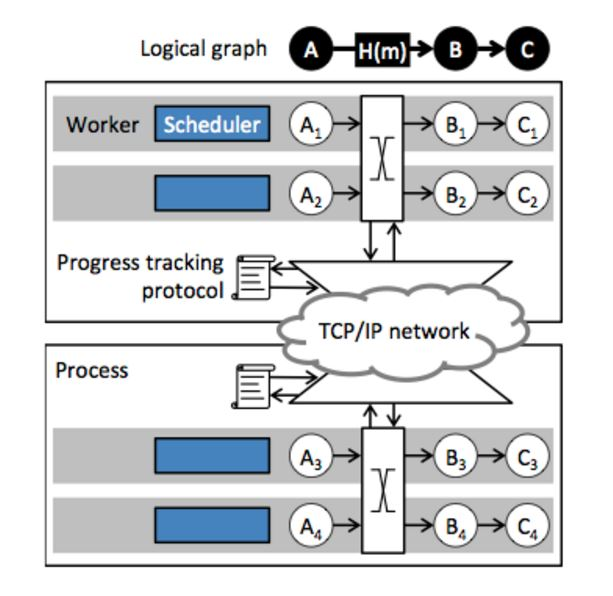
\includegraphics[width=\linewidth]{images/Naiad-Logical_dataflow.JPG}}
\caption{The mapping of a logical dataflow graph onto the distributed
  Naiad system architecture \cite{paper1-Naiad}.}
\label{Naiad-LDF}
\end{figure}

\TODO{Overall, this section is very dense. It would greatly improve
  understanding if you have an example application in mind that you
  relate all the different components of the timely dataflow to.}

\section{System Implementation}
Naiad is high-performance distributed implementation of timely
dataflow and is written in C$\#$, and runs on Windows, Linux, and Mac
OS. Figure \ref{Naiad-LDF} shows the schematic architecture of a Naiad
cluster consisting a group of processes hosting workers that manage a
partition of the timely dataflow vertices \cite{paper3-Naiad}. Each
worker may host several stages of the dataflow graph. The workers are
data nodes and keep a portion of the input data (usually a large-scale
input graph, such as Twitter follower graph) in memory. So it makes
sense to move computation (dataflow graph stages) to the data (the
partitioned input
graph)\cite{www-informationage-blog-wordpress-naiad}. Each process
participates in a distributed progress tracking protocol, in order to
coordinate the delivery of notifications.  All of the features of
C$\#$, including classes, structs, and lambda functions, to build a
timely dataflow graph from a system-provided library of generic Stream
objects can be implemented. Naiad model uses deferred execution
method: like adding a node to internla data flow graph at runtime
while executing a method like Max on a Stream \cite{paper1-Naiad}.

Naiad's distributed implementation also exhibits features like
distributed progress tracking, a simple but extensible implementation
of fault tolerance, high availability, avoidance of micro-straggler
(events like packet loss, contention on concurrent data structures,
and garbage collection which leads to delays ranging from tens of
milliseconds to tens of seconds) which is main obstacle to scalability
for low-latency workloads \cite{paper1-Naiad}.

\section{Performance Evaluation}
Naiad's performance over supporting high-throughput, low latency,
data-parallelism, batch processing, iterative graph data processing
have been examined using several notable micro-benchmarks by Murray
\textit{et al.} \cite{paper1-Naiad} such as Throughput, Latency,
Protocol Optimizations, Scaling. \TODO{Well? What is the conclusion of
  the benchmarks? How does Naiad compare to other systems?}

\section{Use Cases}
Naiad framework has been majorly deployed for batch, streaming and
graph computations serving interactive queries against the results
where Naiad responds to updates and queries with sub-second latencies
\cite{paper1-Naiad}.

\subsection{Batch iterative graph computation}
Implementation of graph algorithms such as PageRank, strongly
connected components (SCC), weakly connected components(WCC), and
approximate shortest path(ASP) in Naiad requires less code complexity
and provides dominant difference in running times compared to PDW
\cite{www-PDW}, DryadLINQ \cite{paper-DryadLINQ},SHS \cite{paper-SHS}
for Category A web graph
\cite{dataset-clueweb09,paper1-Naiad,paper-Largegraphs}.
\subsection{Batch iterative machine learning} Naiad provides competitive platform for custom implementation of distributed machine learning. Also it is straightforward to build communication libraries for existing applications using Naiad’s API. For Eg., modified version of Vowpal Wabbit (VW), an open-source distributed machine learning library which performs iterative linear regression \cite{github-vowpalwabbit}. AllReduce (processes jointly performing global averaging) implementation requires 300 lines of code, around half as many as VW’s AllReduce, and the Naiad code is at a much higher level, abstracting the network sockets and threads being used \cite{paper1-Naiad}.
\subsection{Streaming acyclic computation}
Latency reduction while computing the k-exposure metric for
identifying controversial topics on Twitter using Kineograph, which
takes snapshots of continuosly ingesting graph data for data parallel
computations \cite{paper-Kineograph}.
\subsection{Streaming iterative graph analytics}
Twitter Analysis: To compute the most popular hashtag in each
connected component of the graph of users mentioning other users, and
provide interactive access to the top hashtag in a user’s connected
component.

\section{Useful Resources}
Naiad: A Timely Dataflow System \cite{paper1-Naiad}, provides
extensive study of Naiad's architecture, methodology of working, its
distributed implementation, iterative and incremental data processing,
data analysis applications, comparison with other graph processing
frameworks. Moreover, \cite{github-Naiad}, \cite{www-Nuget},
\cite{paper2-Naiad} are also good resources to learn about Naiad and
programming in Naiad Framework.

\section{Conclusion}
Naiad model enriches \GE dataflow computation with timestamps that
represent logical points in the computation and provide the basis for
an efficient, lightweight coordination mechanism. All the above
capabilities in one package allows development of High-level
programming models on Naiad which can perform tasks as streaming data
analysis, iterative machine learning, and interactive graph
mining. Moreover, it’s \TE public reusable low-level programming
abstractions leads Naiad to outperforms many other data parallel
systems that enforce a single high-level programming model.

\section*{Acknowledgements}

This work was done as part of the course "I524: Big Data and Open
Source Software Projects" at Indiana University during Spring
2017. Many thanks to Professor Gregor von Laszewski and Prof. Geoffrey
Fox at Indiana University Bloomington for their academic as well as
professional guidance. We would also like to thank Associate
Instructors for their help and support during the course.

\bibliography{references}

\end{document}
